
\documentclass[sigconf, screen]{acmart}

\settopmatter{printacmref=false, printccs=false, printfolios=true}
\renewcommand\footnotetextcopyrightpermission[1]{}
\pagestyle{plain}

\usepackage{booktabs}
\usepackage{array}
\usepackage{graphicx}
\usepackage{amsmath}
\usepackage{url}
\graphicspath{{../../figures/}}

% 兜底：任何图都不得超过 0.86 页高。否则 LaTeX 会报
% "Float too large for page" 并把该浮动体无限推迟，引用随之变成 ??。
\setkeys{Gin}{width=\linewidth,height=0.86\textheight,keepaspectratio}

% 放宽浮动体参数：本报告图多（10 张），默认参数会把浮动体排到页外，
% 引发 "Overfull \vbox" 与超大空白页。
\setcounter{topnumber}{4}
\setcounter{bottomnumber}{3}
\setcounter{totalnumber}{7}
\renewcommand{\topfraction}{0.95}
\renewcommand{\bottomfraction}{0.9}
\renewcommand{\textfraction}{0.05}
\renewcommand{\floatpagefraction}{0.80}
\renewcommand{\dbltopfraction}{0.95}
\renewcommand{\dblfloatpagefraction}{0.80}
\setlength{\textfloatsep}{6pt plus 2pt minus 2pt}
\setlength{\floatsep}{6pt plus 2pt minus 2pt}
\setlength{\intextsep}{6pt plus 2pt minus 2pt}

% 双栏窄栏 + 含长不可断词（如 "2,098 / 446 / 446"、"(train/validation/test)"）
% 容易出现 Overfull \hbox。emergencystretch 允许 TeX 在万不得已时拉伸词距，
% 是比 \sloppy 更温和的修法（不会全局放松所有段落的排版）。
\setlength{\emergencystretch}{3em}

\acmConference[]{Technical Report}{October 2026}{}
\acmBooktitle{Technical Report}

\begin{document}

\title{A Controlled Comparison of a Compact CNN and ResNet18 Transfer Learning
for Six-Class SAR Aircraft Classification}

\author{Weiye Pan}
\affiliation{%
  \institution{Independent project repository}
  \country{}}
\email{}

\begin{abstract}
We present a controlled comparison between a compact convolutional neural network
trained from scratch and a ResNet18 model fine-tuned from ImageNet weights for
six-class aircraft classification in synthetic aperture radar (SAR) imagery.
Using the public SAR-ACD dataset (3,032 images, reduced to 2,990
after a duplicate audit), we hold every non-model factor constant: identical
deduplication, an identical stratified split (2,098/446/446),
identical input resolution, normalisation, augmentation, optimisation schedule,
and the same three random seeds. Across three seeds the compact CNN reaches a
macro F1 of 0.6233 $\pm$ 0.0291 while ResNet18 reaches 0.9147 $\pm$ 0.0046, a gain of +0.2913
(significant against the seed-noise threshold of 0.0291). Beyond accuracy,
transfer learning also reduces seed-to-seed variance by roughly 6.3$\times$.
An error analysis shows that a single class pair (A220 $\leftrightarrow$ A320321)
accounts for 52.8\% of all remaining mistakes, and that the two classes
are statistically almost indistinguishable in size and shape. Finally, we quantify
what the model attends to with Grad-CAM, and we deliberately report this evidence
as indicative rather than conclusive, because the dataset provides no bounding
boxes and the aircraft occupies about three quarters of each chip, which limits
the discriminative power of any localisation metric. All numbers in this report
are generated programmatically from the experiment artefacts.
\end{abstract}

\keywords{SAR target classification, transfer learning, ResNet18, Grad-CAM,
reproducibility, error analysis}

\maketitle

% ===========================================================================
\section{Introduction}

Synthetic aperture radar (SAR) provides day-and-night, weather-independent
imaging and is widely used for remote sensing. Recognising aircraft types in SAR
imagery is a challenging fine-grained problem: the targets are small, the imagery
is single-channel and dominated by strong scatterers, and the appearance of a
given aircraft changes drastically with the observation azimuth
\cite{sarsurvey2016}.

This report studies a deliberately simple question: \emph{for a small SAR
aircraft dataset, how much does ImageNet transfer learning actually buy compared
with a compact network trained from scratch, and where does the difference come
from?} We answer it with a controlled experiment rather than a leaderboard entry.
Our contributions are:

\begin{itemize}
\item A \textbf{controlled comparison} in which every factor except the model is
      held fixed, including the random seeds and the data split, so that observed
      differences can be attributed to the model.
\item A \textbf{duplicate audit} performed \emph{before} splitting, which removes
      42 images including 20 cross-class duplicate groups;
      leaving them in place would leak identical images across the train and test
      splits \cite{leakage2012}.
\item An \textbf{error analysis} that localises the residual failures to a single
      aircraft pair, and quantifies how similar the two classes are.
\item A \textbf{critical Grad-CAM analysis}, including an explicit account of why
      the localisation evidence is weaker than it first appears.
\end{itemize}

% ===========================================================================
\section{Dataset}

\subsection{Source and actual statistics}
We use \textbf{SAR-ACD} \cite{saracd2022}, a public six-class civil aircraft
dataset released by the Aerospace Information Research Institute, Chinese Academy
of Sciences. Rather than trusting the published summary, we re-counted the data
locally; Table~\ref{tab:dataset} reports the measured values.

\begin{table}[t]
\caption{Measured dataset statistics, re-computed locally from the 3,032
files rather than copied from the dataset description.}
\label{tab:dataset}
\small
\begin{tabular}{@{}lrrr@{}}
\toprule
Class & Raw & After dedup & Removed \\
\midrule
A220 & 464 & 460 & 4 \\
A320321 & 510 & 498 & 12 \\
A330 & 512 & 501 & 11 \\
ARJ21 & 514 & 513 & 1 \\
Boeing737 & 528 & 528 & 0 \\
Boeing787 & 504 & 490 & 14 \\
\midrule
Total & 3,032 & 2,990 & 42 \\
\bottomrule
\end{tabular}
\end{table}

The images are L (single-channel) JPEGs with variable size
(35--200\,px wide, mean 91.6; 32--150\,px high, mean
83.0); there are 635 distinct size combinations and
0 unreadable files. A fixed input size of 96\,$\times$\,96
was therefore chosen, close to the native median size. The class ratio is
1.148:1, mildly imbalanced, which is why we report macro F1 as the primary
metric. Figure~\ref{fig:eda} summarises the dataset.

\begin{figure}[t]
\centering
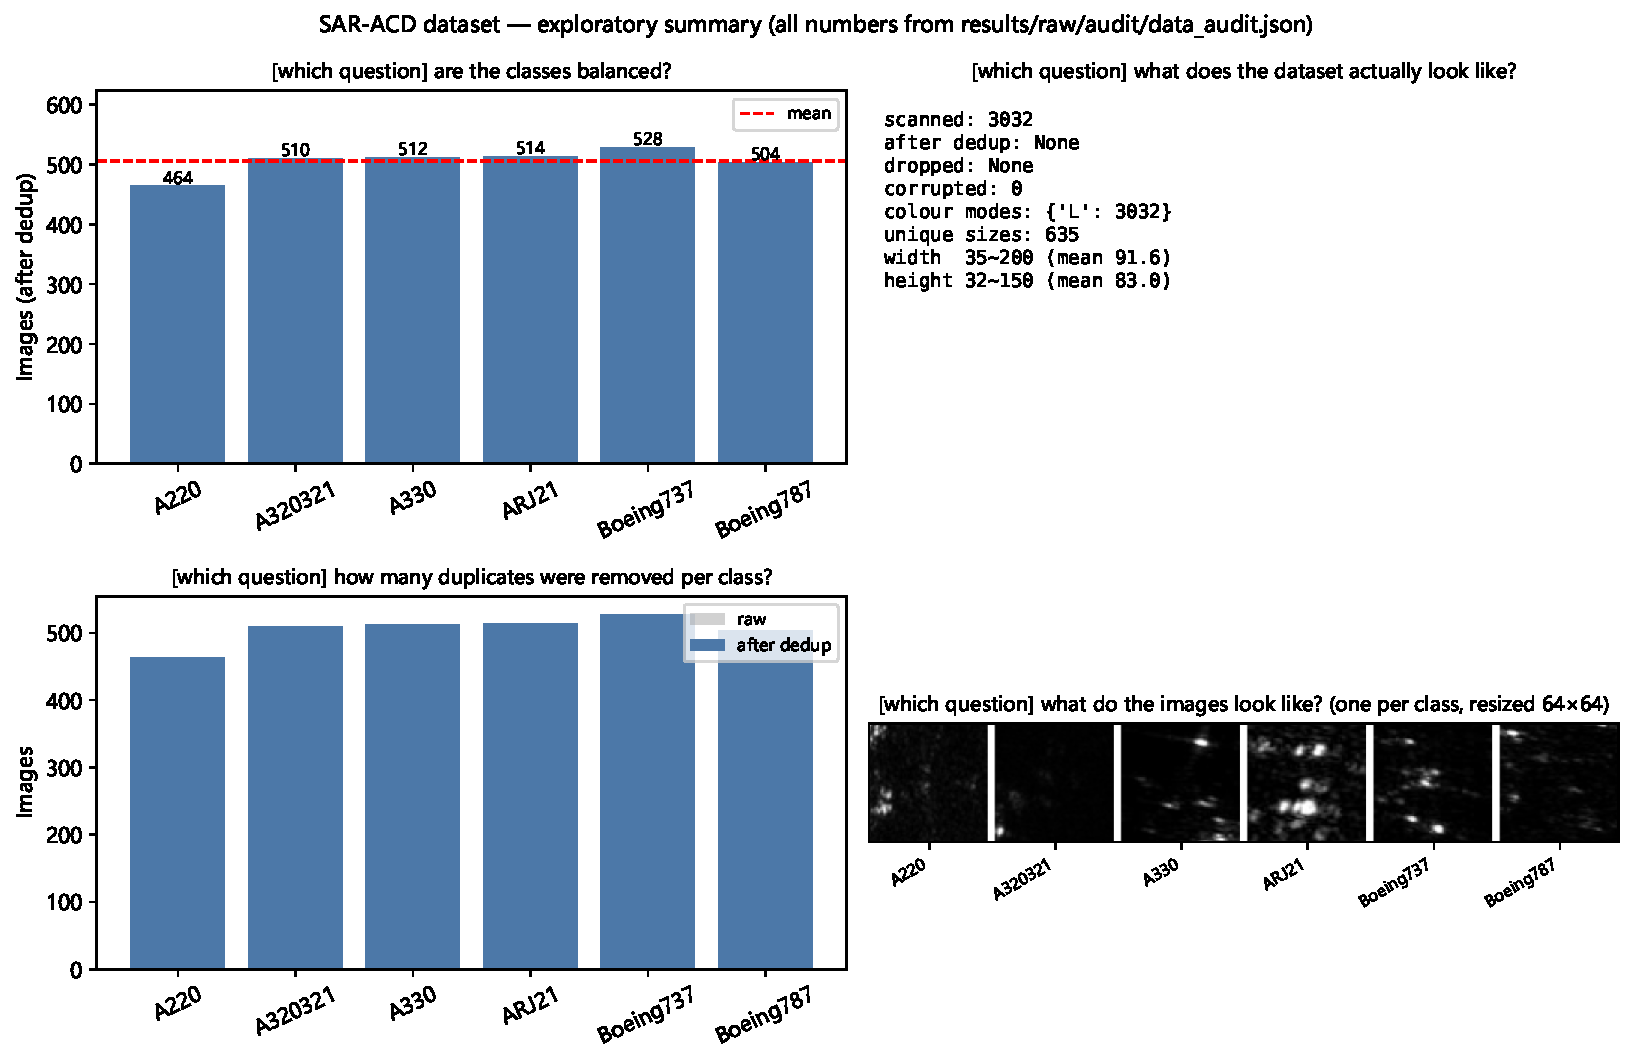
\includegraphics[width=\columnwidth]{cnn_seed42__fig0_data_eda.pdf}
\caption{Dataset overview. All values are read from the audit artefact produced
by the data pipeline; none are transcribed by hand.}
\label{fig:eda}
\end{figure}

\subsection{Duplicate audit and splitting}
A byte-level MD5 audit found 42 exact duplicates in 20
cross-class groups and 2 within-class groups. Cross-class duplicates
are images that appear under two different labels; because no ground truth can
arbitrate them, \emph{both} copies are dropped. Within-class duplicates keep one
copy. Deduplication is performed \textbf{before} splitting: otherwise the same
image could appear in both the training and test sets, silently inflating the test
score \cite{leakage2012}.

The remaining 2,990 images are divided into 2,098 training,
446 validation and 446 test images, using \emph{stratified} sampling
with a fixed seed (42). The split is written to disk and reused by
every model and every seed, so that all runs are compared on identical data.
After splitting, the pipeline asserts that the path sets and the content hashes
of the three subsets are pairwise disjoint, and that the class proportions
deviate by less than one percentage point.

% ===========================================================================
\section{Method}

\subsection{Compact CNN baseline}
The baseline is a four-layer convolutional network designed for
96\,$\times$\,96 single-channel input: four $3\times3$
convolutions (241,382 parameters) with batch normalisation
\cite{batchnorm2015}, $2\times2$ max-pooling after each of the first three,
global average pooling, dropout, and a linear classifier. Because the data are
grayscale, the first convolution takes \textbf{one} input channel; no channel
replication is used for this model.

\subsection{ResNet18 transfer learning}
The second model is ResNet18 \cite{resnet2016} with weights pre-trained on
ImageNet-1k \cite{imagenet2009}, as distributed by \texttt{torchvision}
\cite{pytorch2019}. The final fully connected layer is replaced by a
$\mathrm{Linear}(512 \rightarrow 6)$ layer initialised with a small standard
deviation ($\sigma=0.01$) so that its initially random outputs cannot overwhelm
the pre-trained features.

\textbf{Freezing policy.} We freeze the shallow stages
(\texttt{conv1}, \texttt{bn1}, \texttt{layer1}, \texttt{layer2}) and fine-tune the
deep stages (\texttt{layer3}, \texttt{layer4}) together with the new classifier.
The rationale is that early layers encode generic low-level structure that
transfers, whereas late layers encode task-specific semantics that must adapt;
with only 2,098 training images, updating all 11,179,590 parameters
would be prone to overfitting. The frozen modules are additionally kept in
evaluation mode so that their batch-norm statistics do not drift.

\textbf{Learning rates.} We use discriminative learning rates: $10^{-3}$ for the
new classifier and $10^{-4}$ for the fine-tuned backbone stages
($\approx$10,496,518 trainable parameters, 93.89\% of the model).
Optimisation uses AdamW \cite{adamw2019} with weight decay $10^{-4}$ and a cosine
schedule \cite{sgdr2017}.

\textbf{Grayscale handling.} The dataset yields one-channel images. We replicate
the single channel to three channels inside the model so that \emph{every}
pre-trained weight is used unchanged. The alternative --- rebuilding the first
convolution with one input channel by averaging the pre-trained RGB filters ---
avoids the mismatch between a grayscale input and a colour-pretrained stem, but
introduces an arbitrary averaging step. The replication variant is the more
conservative choice for a transfer-learning study and is what we report.

% ===========================================================================
\section{Experiments}

\subsection{Setup}
All runs use the same pipeline and the same hyper-parameters (Table~\ref{tab:setup}),
differing only in the model. Two deliberate choices deserve emphasis. First, the
normalisation statistics are computed \emph{on the training split only}
(mean 0.0572, std 0.1050) and then applied to validation and test;
computing them on the full dataset would leak information. Second, we deliberately
keep the \emph{same} normalisation for both models instead of using ImageNet
statistics for the pre-trained model: using ImageNet statistics is common practice,
but it would change two factors at once and make the comparison unattributable.

\begin{table}[t]
\caption{Experiment configuration. Every field below is identical for the two
models except the model definition itself.}
\label{tab:setup}
\small
\begin{tabular}{@{}ll@{}}
\toprule
Item & Value \\
\midrule
Input size & 96 $\times$ 96, grayscale \\
Split (train/val/test) & 2,098 / 446 / 446, seed 42 \\
Augmentation & rotation $\pm30^\circ$, flip, translate 5\%, scale 0.9--1.1 \\
 & (training split only) \\
Optimiser & AdamW, weight decay 1e-4 \\
Learning rate & CNN 1e-3; ResNet18 head 1e-3 / backbone 1e-4 \\
Schedule & cosine annealing \\
Epochs / batch & 40 / 64 \\
Early stopping & validation macro F1, patience 10 \\
Random seeds & 42, 123, 2024 \\
Model selection & best \emph{validation} macro F1 \\
\bottomrule
\end{tabular}
\end{table}

\subsection{Metrics and protocol}
We report accuracy, macro F1 (primary), weighted F1, per-class
precision/recall/F1, and confusion matrices (raw and row-normalised). The test
split is evaluated \emph{once} per run, using the checkpoint selected on the
validation split; no test-set quantity is used for any decision. Each evaluation
appends a record to a ledger, so the number of test-set evaluations is auditable.
Every configuration is run with 42, 123, 2024 seeds and we report means and standard
deviations.

\subsection{Training behaviour}
Figures~\ref{fig:curvescnn} and~\ref{fig:curvesrn} show the training curves of all
three seeds for the two models. The baseline converges slowly and its validation
score keeps fluctuating; ResNet18 reaches a much higher level within a few epochs
and its three seeds nearly coincide.

\begin{figure}[t]
\centering
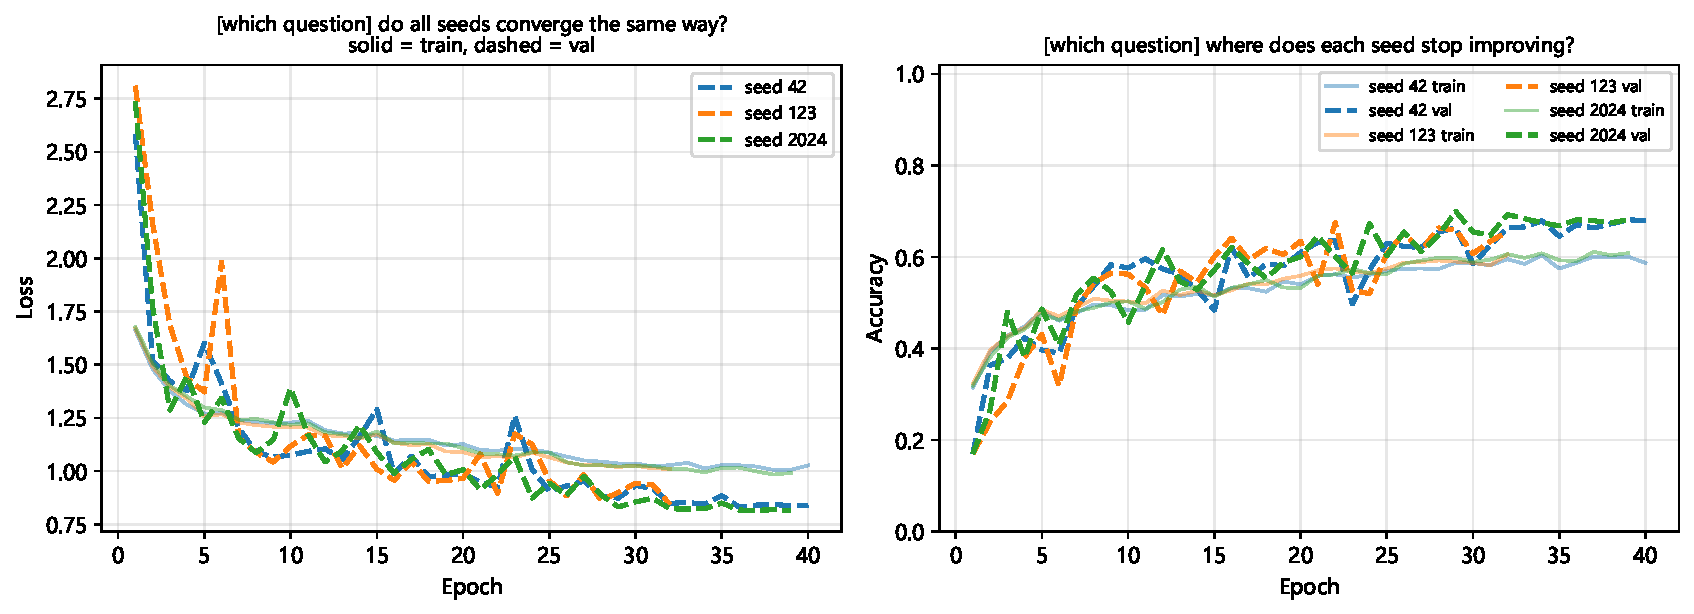
\includegraphics[width=\columnwidth]{cnn_baseline__fig1c_train_curves_all_seeds.pdf}
\caption{Compact CNN: loss and accuracy for the three seeds (solid = train,
dashed = validation). The seeds diverge noticeably.}
\label{fig:curvescnn}
\end{figure}

\begin{figure}[t]
\centering
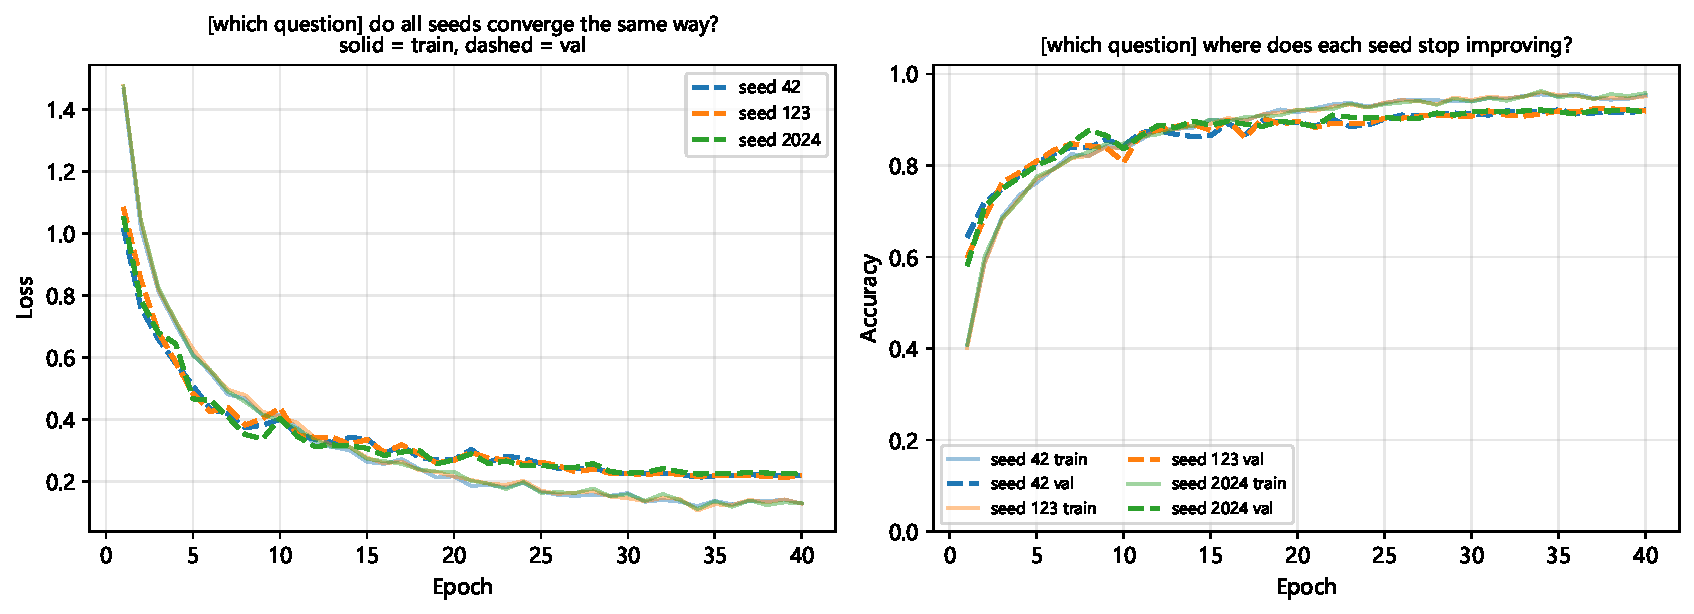
\includegraphics[width=\columnwidth]{resnet18_transfer__fig1c_train_curves_all_seeds.pdf}
\caption{ResNet18 transfer learning: the three seeds track each other closely,
indicating a much more stable optimisation.}
\label{fig:curvesrn}
\end{figure}

% ===========================================================================
\section{Results}

\subsection{Overall comparison}
Table~\ref{tab:results} reports the test-set results. ResNet18 improves macro F1
by +0.2913, from 0.6233 $\pm$ 0.0291 to 0.9147 $\pm$ 0.0046, a relative gain of 46.7\%.
Figure~\ref{fig:cmp} shows the same comparison graphically.

Following the protocol fixed before the experiments, we only call a difference
meaningful when the gap in means exceeds the larger of the two standard
deviations. Here the gap (+0.2913) is about an order of magnitude larger than the
threshold (0.0291), so the improvement is \textbf{significant}. A second, easily
overlooked result is that transfer learning also makes the outcome far more
reproducible: the macro-F1 standard deviation drops from 0.6329, 0.5839, 0.6532's spread to
a spread of 0.9081, 0.9182, 0.9177 across seeds, a reduction of about 6.3$\times$.

\begin{table}[t]
\caption{Test-set results (mean $\pm$ std over 42, 123, 2024 seeds). The seed-noise
threshold is 0.0291; a difference counts as meaningful only if it exceeds it.
All three differences do.}
\label{tab:results}
\small
\begin{tabular}{@{}lccc@{}}
\toprule
Metric & Compact CNN & ResNet18 & $\Delta$ \\
\midrule
Accuracy & 0.6293 $\pm$ 0.0274 & 0.9163 $\pm$ 0.0042 & +0.2870 \\
Macro F1 & 0.6233 $\pm$ 0.0291 & 0.9147 $\pm$ 0.0046 & +0.2913 \\
Weighted F1 & 0.6250 $\pm$ 0.0295 & 0.9165 $\pm$ 0.0045 & +0.2915 \\
\bottomrule
\end{tabular}
\end{table}

\begin{figure}[t]
\centering
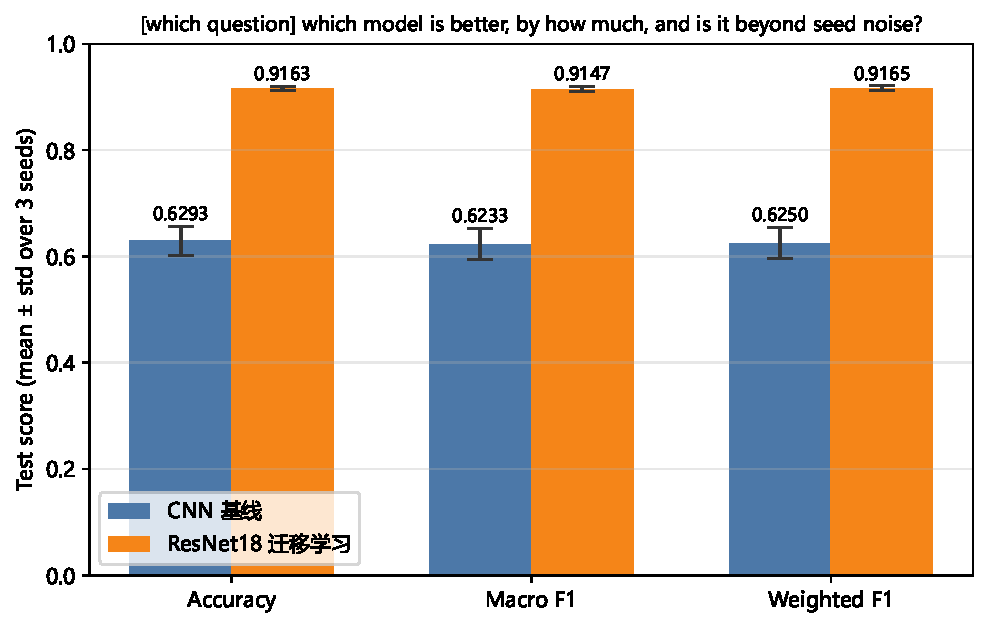
\includegraphics[width=\columnwidth]{comparison_cnn_baseline_vs_resnet18_transfer__fig6a_model_comparison.pdf}
\caption{Overall test metrics. Error bars are standard deviations over the
42, 123, 2024 seeds; annotations give the delta and whether it exceeds the seed noise.}
\label{fig:cmp}
\end{figure}

\subsection{Per-class behaviour}
Table~\ref{tab:perclass} and Figure~\ref{fig:perclass} break the result down by
class. The improvement is not uniform. The largest gains occur precisely in the
classes the baseline struggled with most, while the smallest gain is on A320321.

\begin{table}[t]
\caption{Per-class F1 (mean over 42, 123, 2024 seeds), sorted by improvement.}
\label{tab:perclass}
\small
\begin{tabular}{@{}lcccc@{}}
\toprule
Class & Support & CNN & ResNet18 & $\Delta$ \\
\midrule
Boeing787 & 73 & 0.5892 & 0.9818 & +0.3926 \\
Boeing737 & 79 & 0.6202 & 0.9642 & +0.3440 \\
A330 & 75 & 0.6632 & 0.9626 & +0.2994 \\
A220 & 69 & 0.5220 & 0.8213 & +0.2993 \\
ARJ21 & 76 & 0.7158 & 0.9662 & +0.2504 \\
A320321 & 74 & 0.6294 & 0.7918 & +0.1624 \\
\bottomrule
\end{tabular}
\end{table}

\begin{figure}[t]
\centering
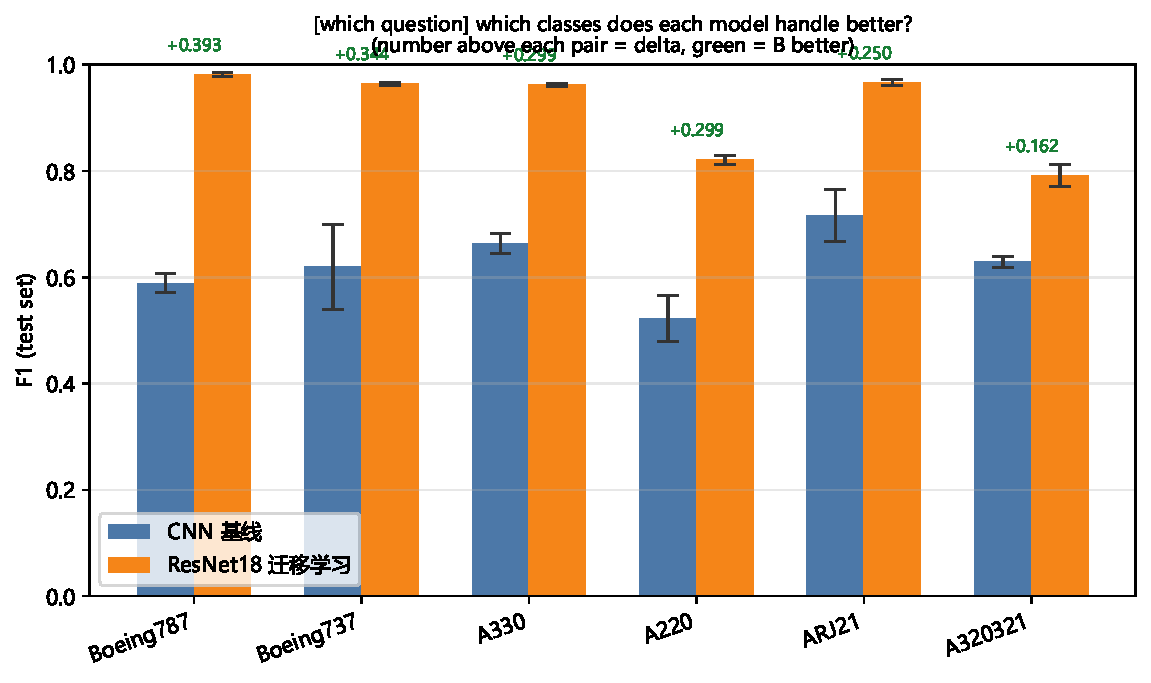
\includegraphics[width=\columnwidth]{comparison_cnn_baseline_vs_resnet18_transfer__fig6b_per_class_f1.pdf}
\caption{Per-class F1 for both models, ordered by improvement.}
\label{fig:perclass}
\end{figure}

\subsection{Confusion structure}
Figure~\ref{fig:cm} contrasts the row-normalised confusion matrices. The baseline
makes mistakes in many directions at once, whereas ResNet18 is close to diagonal
everywhere except for one pair of classes, which we examine next.

\begin{figure*}[t]
\centering
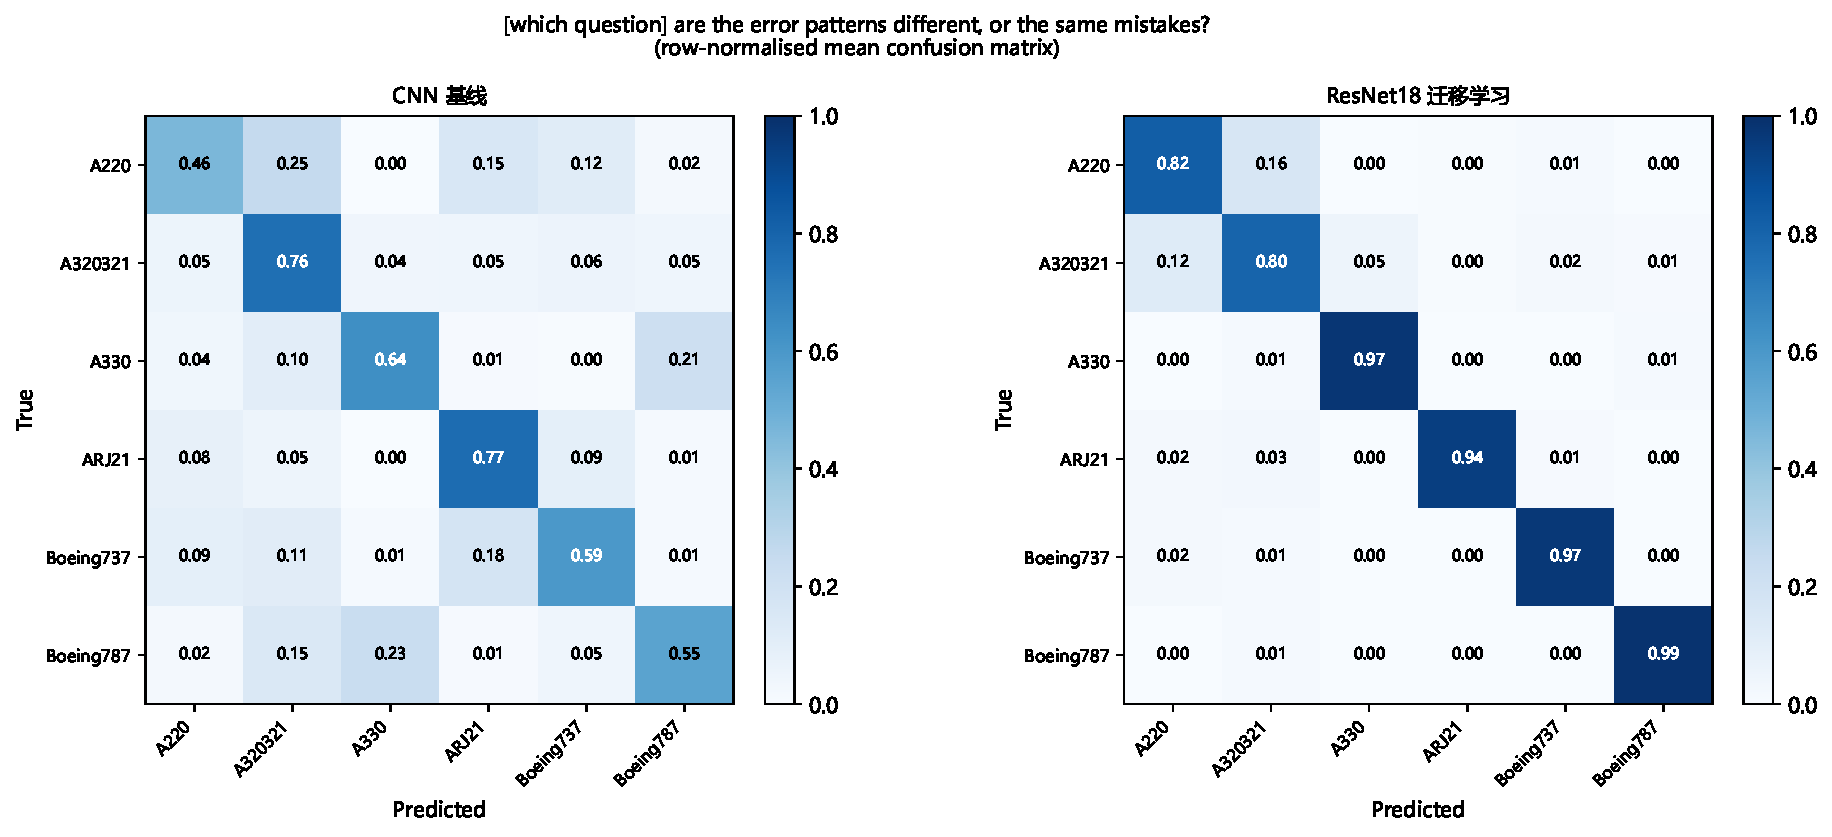
\includegraphics[width=0.86\textwidth]{comparison_cnn_baseline_vs_resnet18_transfer__fig6d_confusion_side_by_side.pdf}
\caption{Row-normalised confusion matrices (mean over 42, 123, 2024 seeds).
Left: compact CNN. Right: ResNet18. The baseline errs in several directions;
ResNet18 leaves essentially a single confused pair.}
\label{fig:cm}
\end{figure*}

% ===========================================================================
\section{Error Analysis}

\subsection{Final model and error sample set}
The final model is chosen \textbf{on validation performance only}: we first pick
the better model family by mean validation macro F1 (ResNet18 0.9199
$\pm$ 0.0011 versus the baseline 0.6802 $\pm$ 0.0118), then
the best seed within that family (seed 123, validation macro F1
0.9215). No test-set quantity takes part in this selection.

On the test split the final model makes 36 errors out of 446
(8.07\%). \textbf{All} of them are visualised in Figure~\ref{fig:wrong};
none are discarded. Errors are less confident than correct predictions
(0.760 versus 0.958, a gap of 0.198), which suggests that a
confidence threshold could be used for rejection in deployment.

\begin{figure*}[t]
\centering
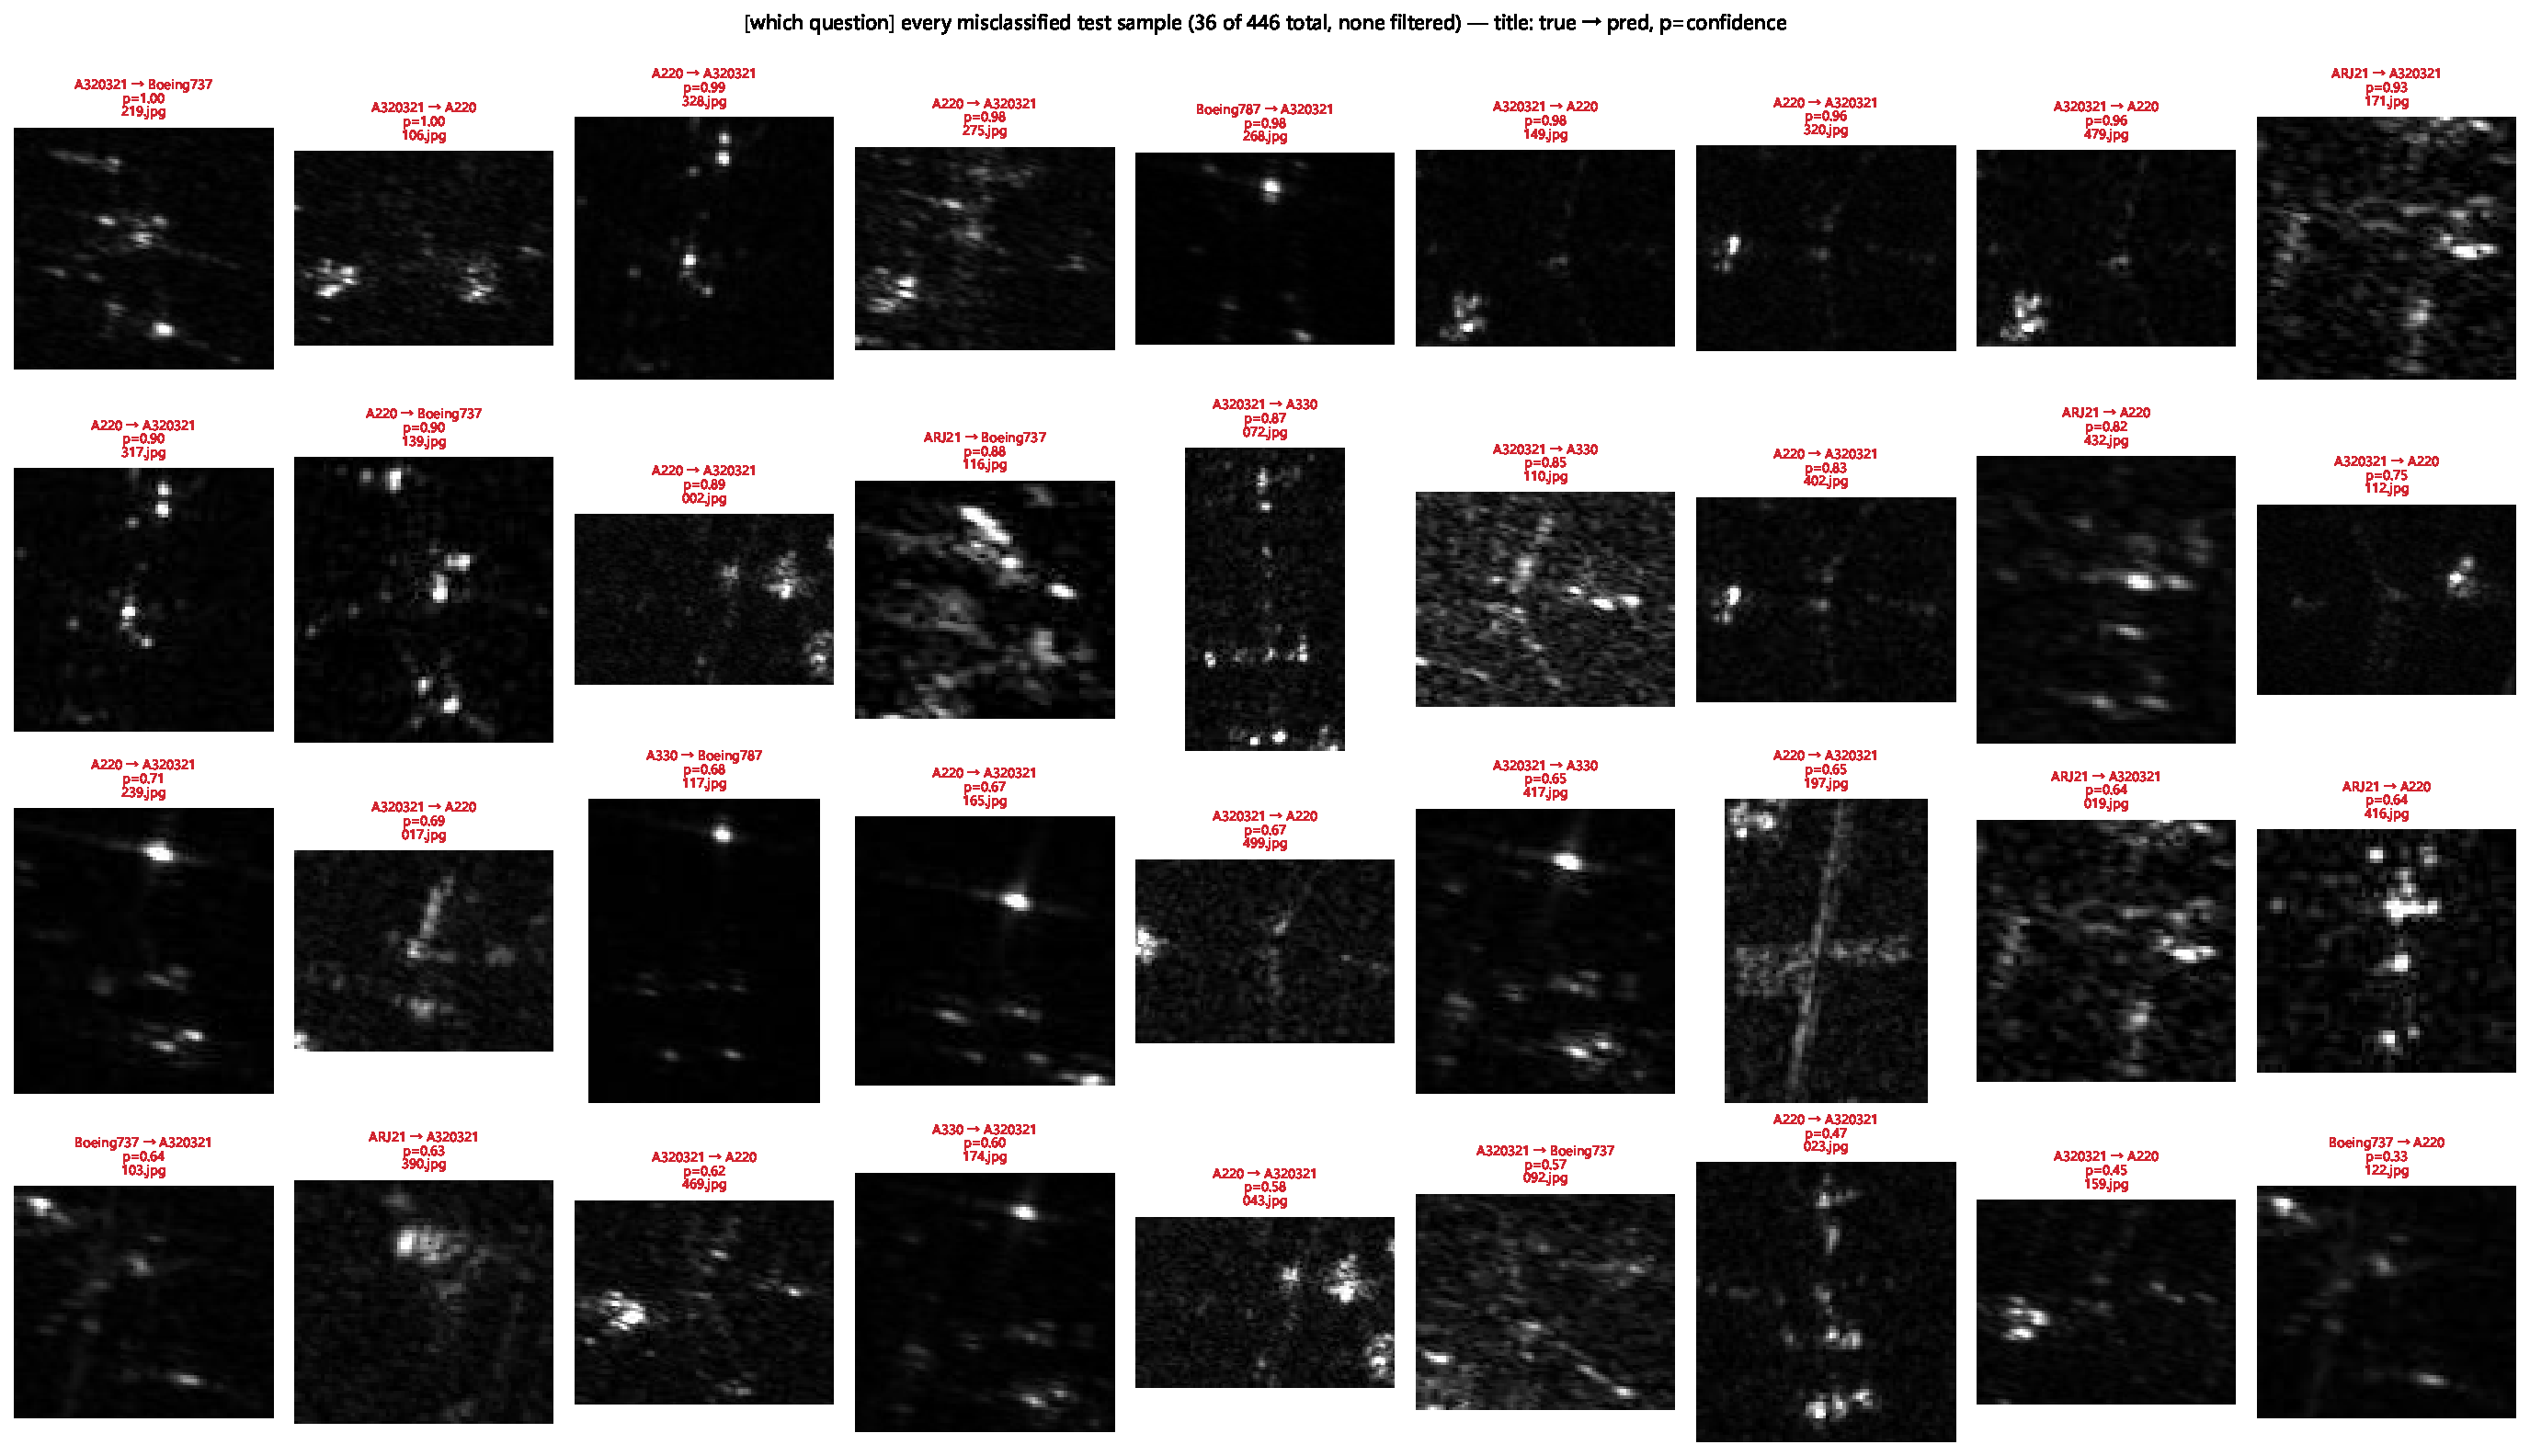
\includegraphics[width=0.86\textwidth]{error_analysis__fig7a_all_wrong_samples.pdf}
\caption{Every misclassified test image (36 of 446). Titles give
true class $\rightarrow$ predicted class and the predicted confidence. No
sample is filtered out.}
\label{fig:wrong}
\end{figure*}

\subsection{The dominant confusion}
Table~\ref{tab:errdir} lists the error directions. A single pair dominates:
A220 $\leftrightarrow$ A320321 accounts for 52.8\% of all errors and is
\emph{bidirectional} (0.159 of true A220 predicted as A320321, and
0.108 in the opposite direction), which indicates genuine overlap in feature
space rather than one class being absorbed by another.

\begin{table}[t]
\caption{Most frequent error directions of the final model.}
\label{tab:errdir}
\small
\begin{tabular}{@{}lrrr@{}}
\toprule
True $\rightarrow$ Pred. & Count & Share & Mean conf. \\
\midrule
A220 $\rightarrow$ A320321 & 11 & 30.6\% & 0.785 \\
A320321 $\rightarrow$ A220 & 8 & 22.2\% & 0.765 \\
ARJ21 $\rightarrow$ A320321 & 3 & 8.3\% & 0.734 \\
A320321 $\rightarrow$ A330 & 3 & 8.3\% & 0.789 \\
A320321 $\rightarrow$ Boeing737 & 2 & 5.6\% & 0.785 \\
ARJ21 $\rightarrow$ A220 & 2 & 5.6\% & 0.730 \\
\bottomrule
\end{tabular}
\end{table}

\subsection{Why are these two classes confused?}
Table~\ref{tab:shape} compares measurable properties of the two classes. Every
statistic differs by less than 16.6\%, i.e. the two aircraft are
nearly indistinguishable by size and shape statistics alone. Together with the
bidirectionality of the errors, this supports three explanations, in decreasing
order of evidential support:

\begin{enumerate}
\item \textbf{Genuine shape similarity.} A220 and A320321 are both narrow-body
      airliners; at the resolution available here, their wing sweep, engine
      layout and fuselage proportions differ little.
\item \textbf{Azimuth variation masquerading as class variation.} SAR scattering
      is extremely azimuth-sensitive: the same aircraft seen from different
      aspects can differ more than two different aircraft seen from the same
      aspect. Random rotation augmentation ($\pm30^\circ$, applied here) may
      additionally blur this boundary.
\item \textbf{Insufficient resolution.} Resizing to 96\,$\times$\,96
      discards detail; the native chips are only about 91.6\,$\times$\,83.0\,px.
\end{enumerate}

\begin{table}[t]
\caption{Measured properties of the confused pair (medians unless noted).
All relative differences are below 16.6\%.}
\label{tab:shape}
\small
\begin{tabular}{@{}lccc@{}}
\toprule
Statistic & A220 & A320321 & Rel. diff. \\
\midrule
image width (median, px) & 82 & 92 & 11.5\% \\
image height (median, px) & 72 & 78 & 8.0\% \\
aspect ratio (median) & 1.137 & 1.238 & 8.5\% \\
bright-target area fraction & 0.724 & 0.832 & 13.8\% \\
mean image brightness & 17.4 & 14.8 & 16.6\% \\
\bottomrule
\end{tabular}
\end{table}

\begin{figure}[t]
\centering
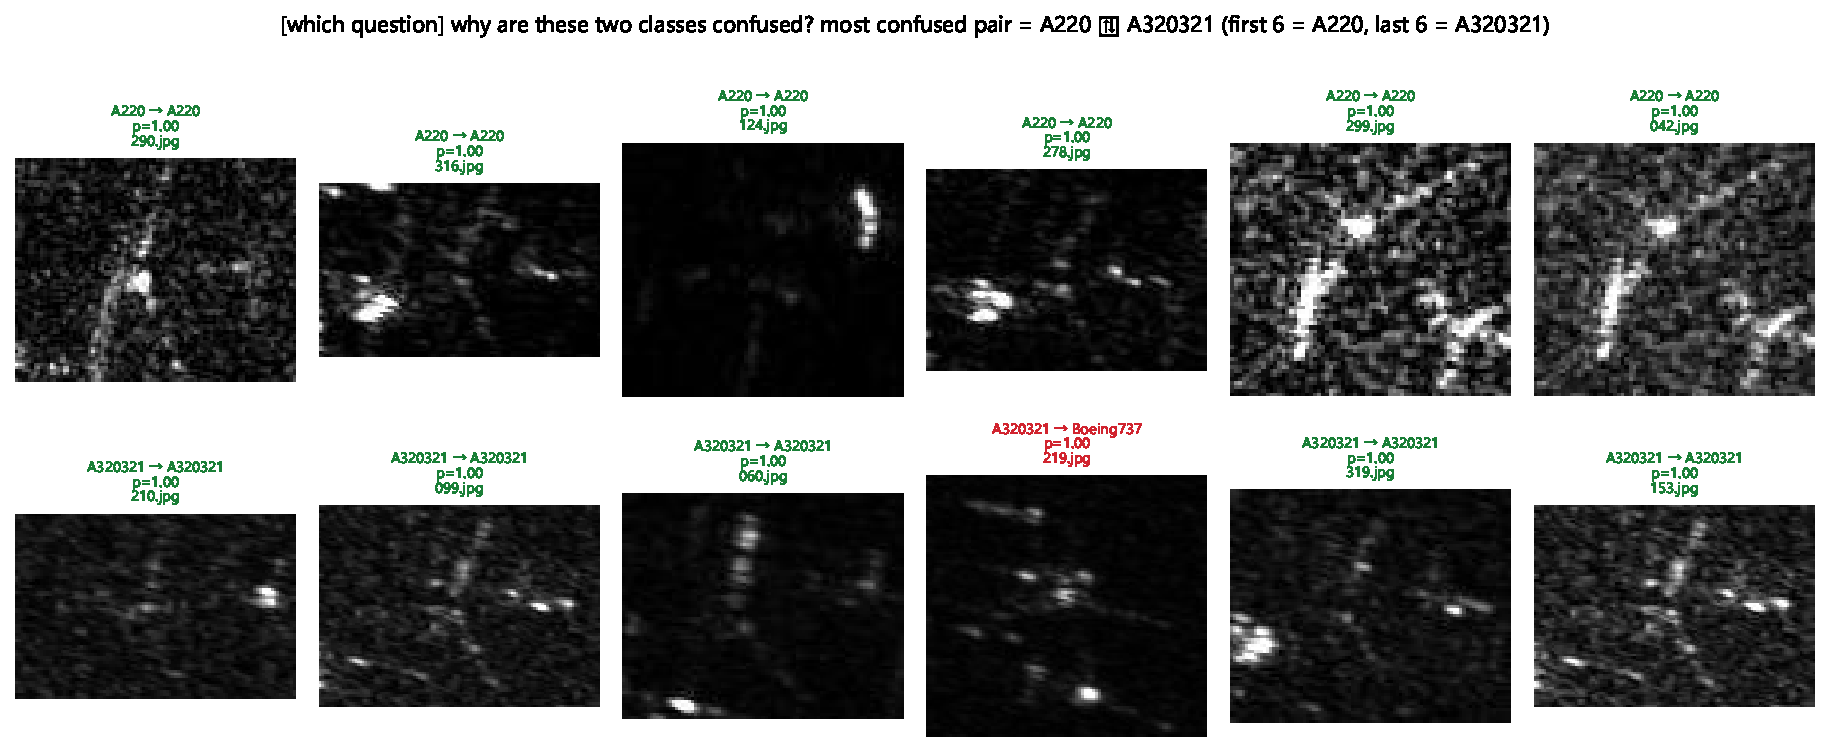
\includegraphics[width=\columnwidth]{error_analysis__fig7d_most_confused_pair.pdf}
\caption{The most confused pair. First six images are true A220, the last six
true A320321; titles give true $\rightarrow$ predicted and confidence.}
\label{fig:pair}
\end{figure}

The first two explanations are \emph{inferences} consistent with the evidence, not
established facts; confirming them would require azimuth metadata per image or
target boxes for alignment.

% ===========================================================================
\section{Grad-CAM Interpretability}

\subsection{How the measurement is made}
This dataset has no bounding boxes, so we approximate the target region by the
pixels brighter than $\mu+\sigma$ (SAR aircraft are strong scatterers). We then
measure the fraction of Grad-CAM \cite{gradcam2017} mass that falls on those
pixels and compare it with the fraction that a random heat map would produce.

A methodological finding is important here. Our first measurement suggested an
essentially random localisation. The cause was resolution, not indifference:
ResNet18 downsamples by a factor of 32, so on 96\,$\times$\,96
inputs the \texttt{layer4} feature map is only
3×3 (each cell spanning 32\,$\times$\,32 pixels of the input).
Table~\ref{tab:cam} therefore also reports \texttt{layer3}
(6×6), and Figure~\ref{fig:camloc} shows both.

\begin{table}[t]
\caption{Grad-CAM localisation by target layer. ``Lift'' is the ratio of CAM mass
on bright pixels to the random baseline.}
\label{tab:cam}
\small
\begin{tabular}{@{}lcccc@{}}
\toprule
Layer & CAM grid & On target & Random & Lift \\
\midrule
\texttt{layer3} & 6×6 & 0.0878 & 0.0653 & 1.34$\times$ \\
\texttt{layer4} & 3×3 & 0.0774 & 0.0653 & 1.18$\times$ \\
\bottomrule
\end{tabular}
\end{table}

\subsection{What the model attends to}
Using the finer \texttt{layer3} layer, 0.0878 of the CAM mass falls
on bright target pixels against a random baseline of 0.0653, a lift of
\textbf{1.34}$\times$. The same quantity is 0.0887 for correct
predictions and 0.0770 for incorrect ones. Figure~\ref{fig:camloc} shows the
distribution and the layer comparison; Figure~\ref{fig:camx} contrasts the most
target-focused and the most diffuse examples.

\begin{figure}[t]
\centering
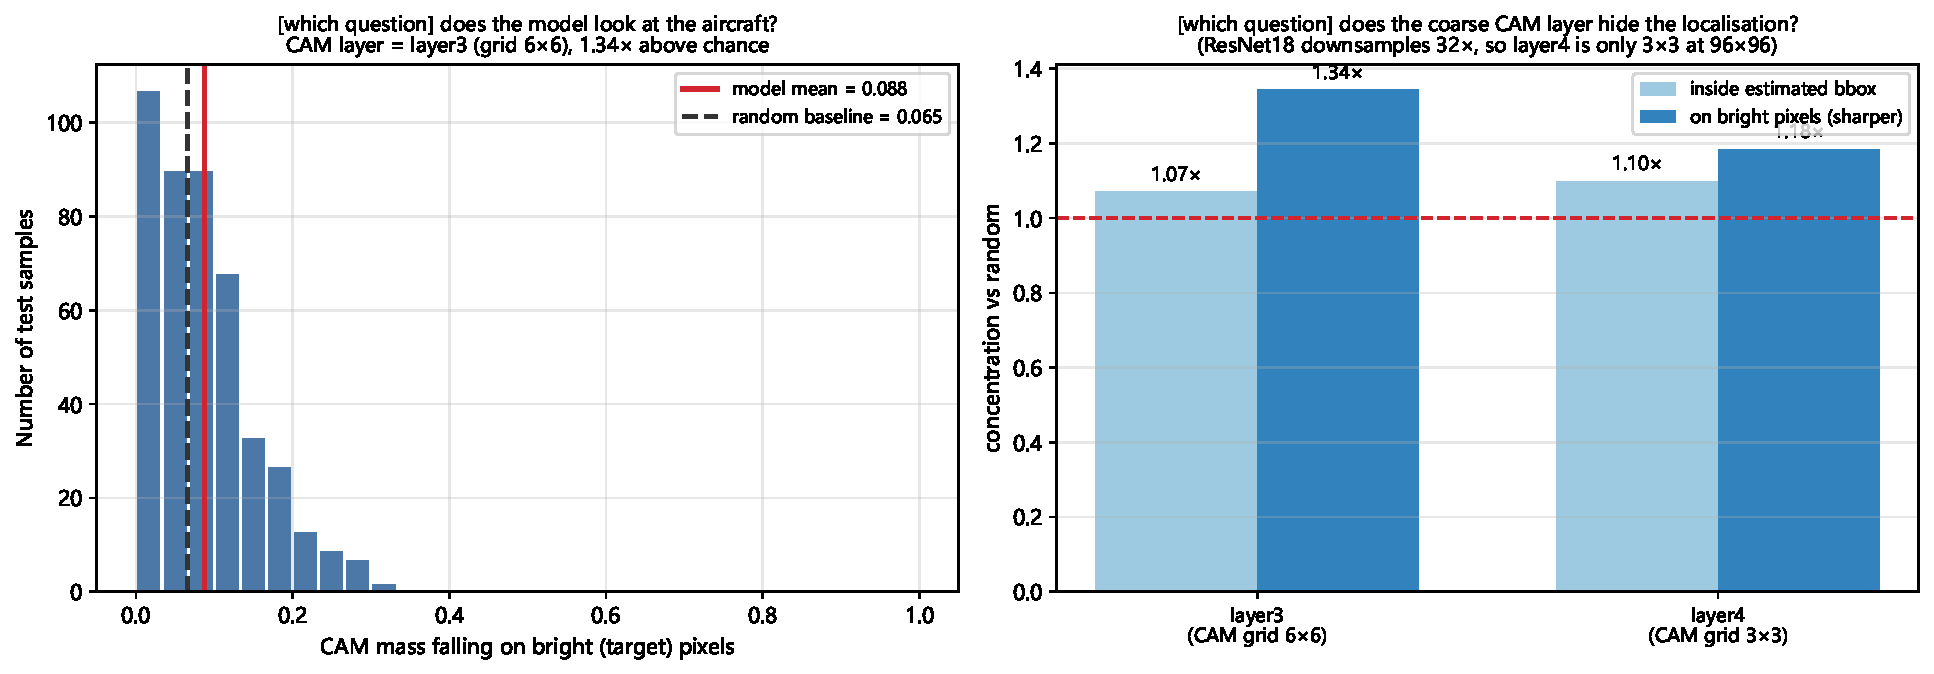
\includegraphics[width=\columnwidth]{error_analysis__fig7e_cam_localization.pdf}
\caption{Left: distribution of CAM mass landing on bright target pixels
(\texttt{layer3}), with the random baseline. Right: concentration
relative to chance for both candidate layers, showing that the coarse
\texttt{layer4} map understates the localisation.}
\label{fig:camloc}
\end{figure}

\begin{figure}[t]
\centering
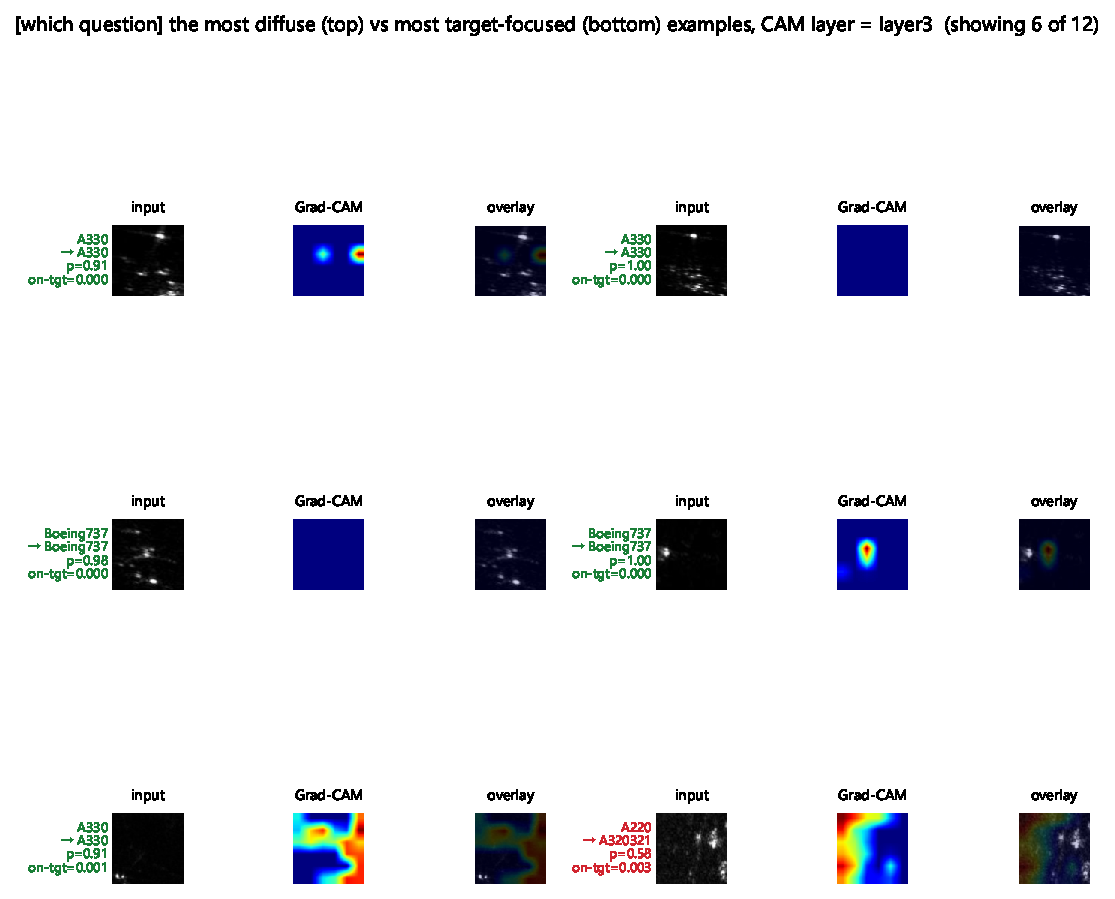
\includegraphics[width=\columnwidth]{error_analysis__fig7f_cam_on_vs_off_target.pdf}
\caption{The most target-focused (bottom) and most diffuse (top) examples for
\texttt{layer3}.}
\label{fig:camx}
\end{figure}

We deliberately stop short of claiming that the model ``looks at the aircraft''.
A lift of 1.34$\times$ is a tendency, not a decisive result, and the
measurement has three limitations: (i) the target region is approximated by
bright pixels rather than annotated, so strong sidelobes count as target;
(ii) the aircraft occupies roughly three quarters of each chip, which leaves
little room for a background-driven model and makes any localisation metric
intrinsically weak; and (iii) even 6×6 is a coarse grid. We therefore
report this section as \emph{indicative evidence}.

% ===========================================================================
\section{Limitations}

\paragraph{The public subset contains expanded samples.}
The released portion of SAR-ACD is described by its authors as
``3,032 images in six civilian categories \emph{after expansion}''.
Augmented or synthetically enlarged samples can share near-duplicate structure
with the originals. Although our byte-level audit removed exact duplicates, it
cannot detect near-duplicates created by augmentation, so the reported test
scores should be read as an \emph{upper bound} for genuinely unseen data.

\paragraph{Results do not establish cross-airport generalisation.}
The imagery covers the Shanghai Hongqiao airport area and a small number of other
airports, acquired at particular times and geometries. Several classes may be
correlated with the acquisition site or the flight schedule rather than with the
aircraft shape. Our evaluation is a random split within this collection, so it
measures \emph{within-collection} generalisation only. Nothing here supports a
claim about performance at a new airport, a new sensor, or a new frequency band.

\paragraph{Other limitations.}
The dataset has no bounding boxes, so localisation evidence remains indirect
(Section~7) and target-aligned comparisons are impossible. The images are
single-polarisation and single-channel, so polarimetric or multi-look cues are
unavailable. Finally, three seeds are the minimum needed to estimate spread; the
resulting standard deviations are indicative rather than precise.

% ===========================================================================
\section{Conclusion and Future Work}

In a fully controlled comparison on six-class SAR aircraft classification,
ImageNet transfer learning improved macro F1 from 0.6233 $\pm$ 0.0291 to 0.9147 $\pm$ 0.0046
(+0.2913) while reducing seed-to-seed variance by roughly 6.3$\times$.
The residual errors are highly concentrated: A220 $\leftrightarrow$ A320321 alone
accounts for 52.8\% of them, and the two classes are statistically
almost identical in size and shape. A critical Grad-CAM analysis indicates that
the model is more target-focused than chance, but we report that as a tendency
rather than a conclusion, and we explain why the measurement cannot be stronger
with the data available.

Future work, in priority order:
\begin{itemize}
\item \textbf{Resolve the dominant confusion.} If azimuth metadata can be
      recovered, stratify the error rate by aspect angle; otherwise, obtain
      target boxes and evaluate after alignment, so that shape rather than
      pose is compared.
\item \textbf{Near-duplicate detection.} Replace exact-hash auditing with
      perceptual hashing or embedding-based deduplication to bound the effect of
      the expanded public subset.
\item \textbf{Cross-airport evaluation.} Partition by acquisition site and report
      leave-one-site-out accuracy, which is the claim that actually matters for
      deployment.
\item \textbf{Freezing-policy ablation.} The implementation already supports
      full fine-tuning and linear probing; comparing them would separate
      ``pre-training helps'' from ``more parameters help''.
\item \textbf{Resolution study.} Repeat at 96 and at higher input sizes to
      test whether the A220/A320321 boundary is limited by resolution.
\end{itemize}

\section*{Reproducibility}
Every number, table and figure in this report is generated programmatically from
the artefacts under \texttt{results/}. The split is fixed by seed 42 and
asserted to be leakage-free; each test-set evaluation is recorded in a ledger; and
each run stores its resolved configuration, log, per-epoch history, metrics and
checkpoint. A clean-room reproduction consists of cloning the repository, creating
the environment from \texttt{environment.yml}, and running the pipeline scripts in
order.

\bibliographystyle{ACM-Reference-Format}
\bibliography{refs}

\end{document}
